% !TEX encoding = UTF-8
% !TEX TS-program = pdflatex
% !TEX root = ../../tesi.tex

\section{Libreria per l'integrazione con gli smart contract}
La libreria per l'integrazione con i contratti ha lo scopo di permettere al \textit{back-end}, sviluppato con Spring, di comunicare con i contratti caricati nelle \textit{blockchain}.

\subsection{Progettazione}
A partire da quanto richiesto dall'analisi dei requisiti, ho basato la soluzione progettuale della libreria per l'integrazione con gli \textit{smart contract} sulle \textit{best practices} del linguaggio Java e sui principi \textit{SOLID}.

\begin{figure}[h!]
  \centering
  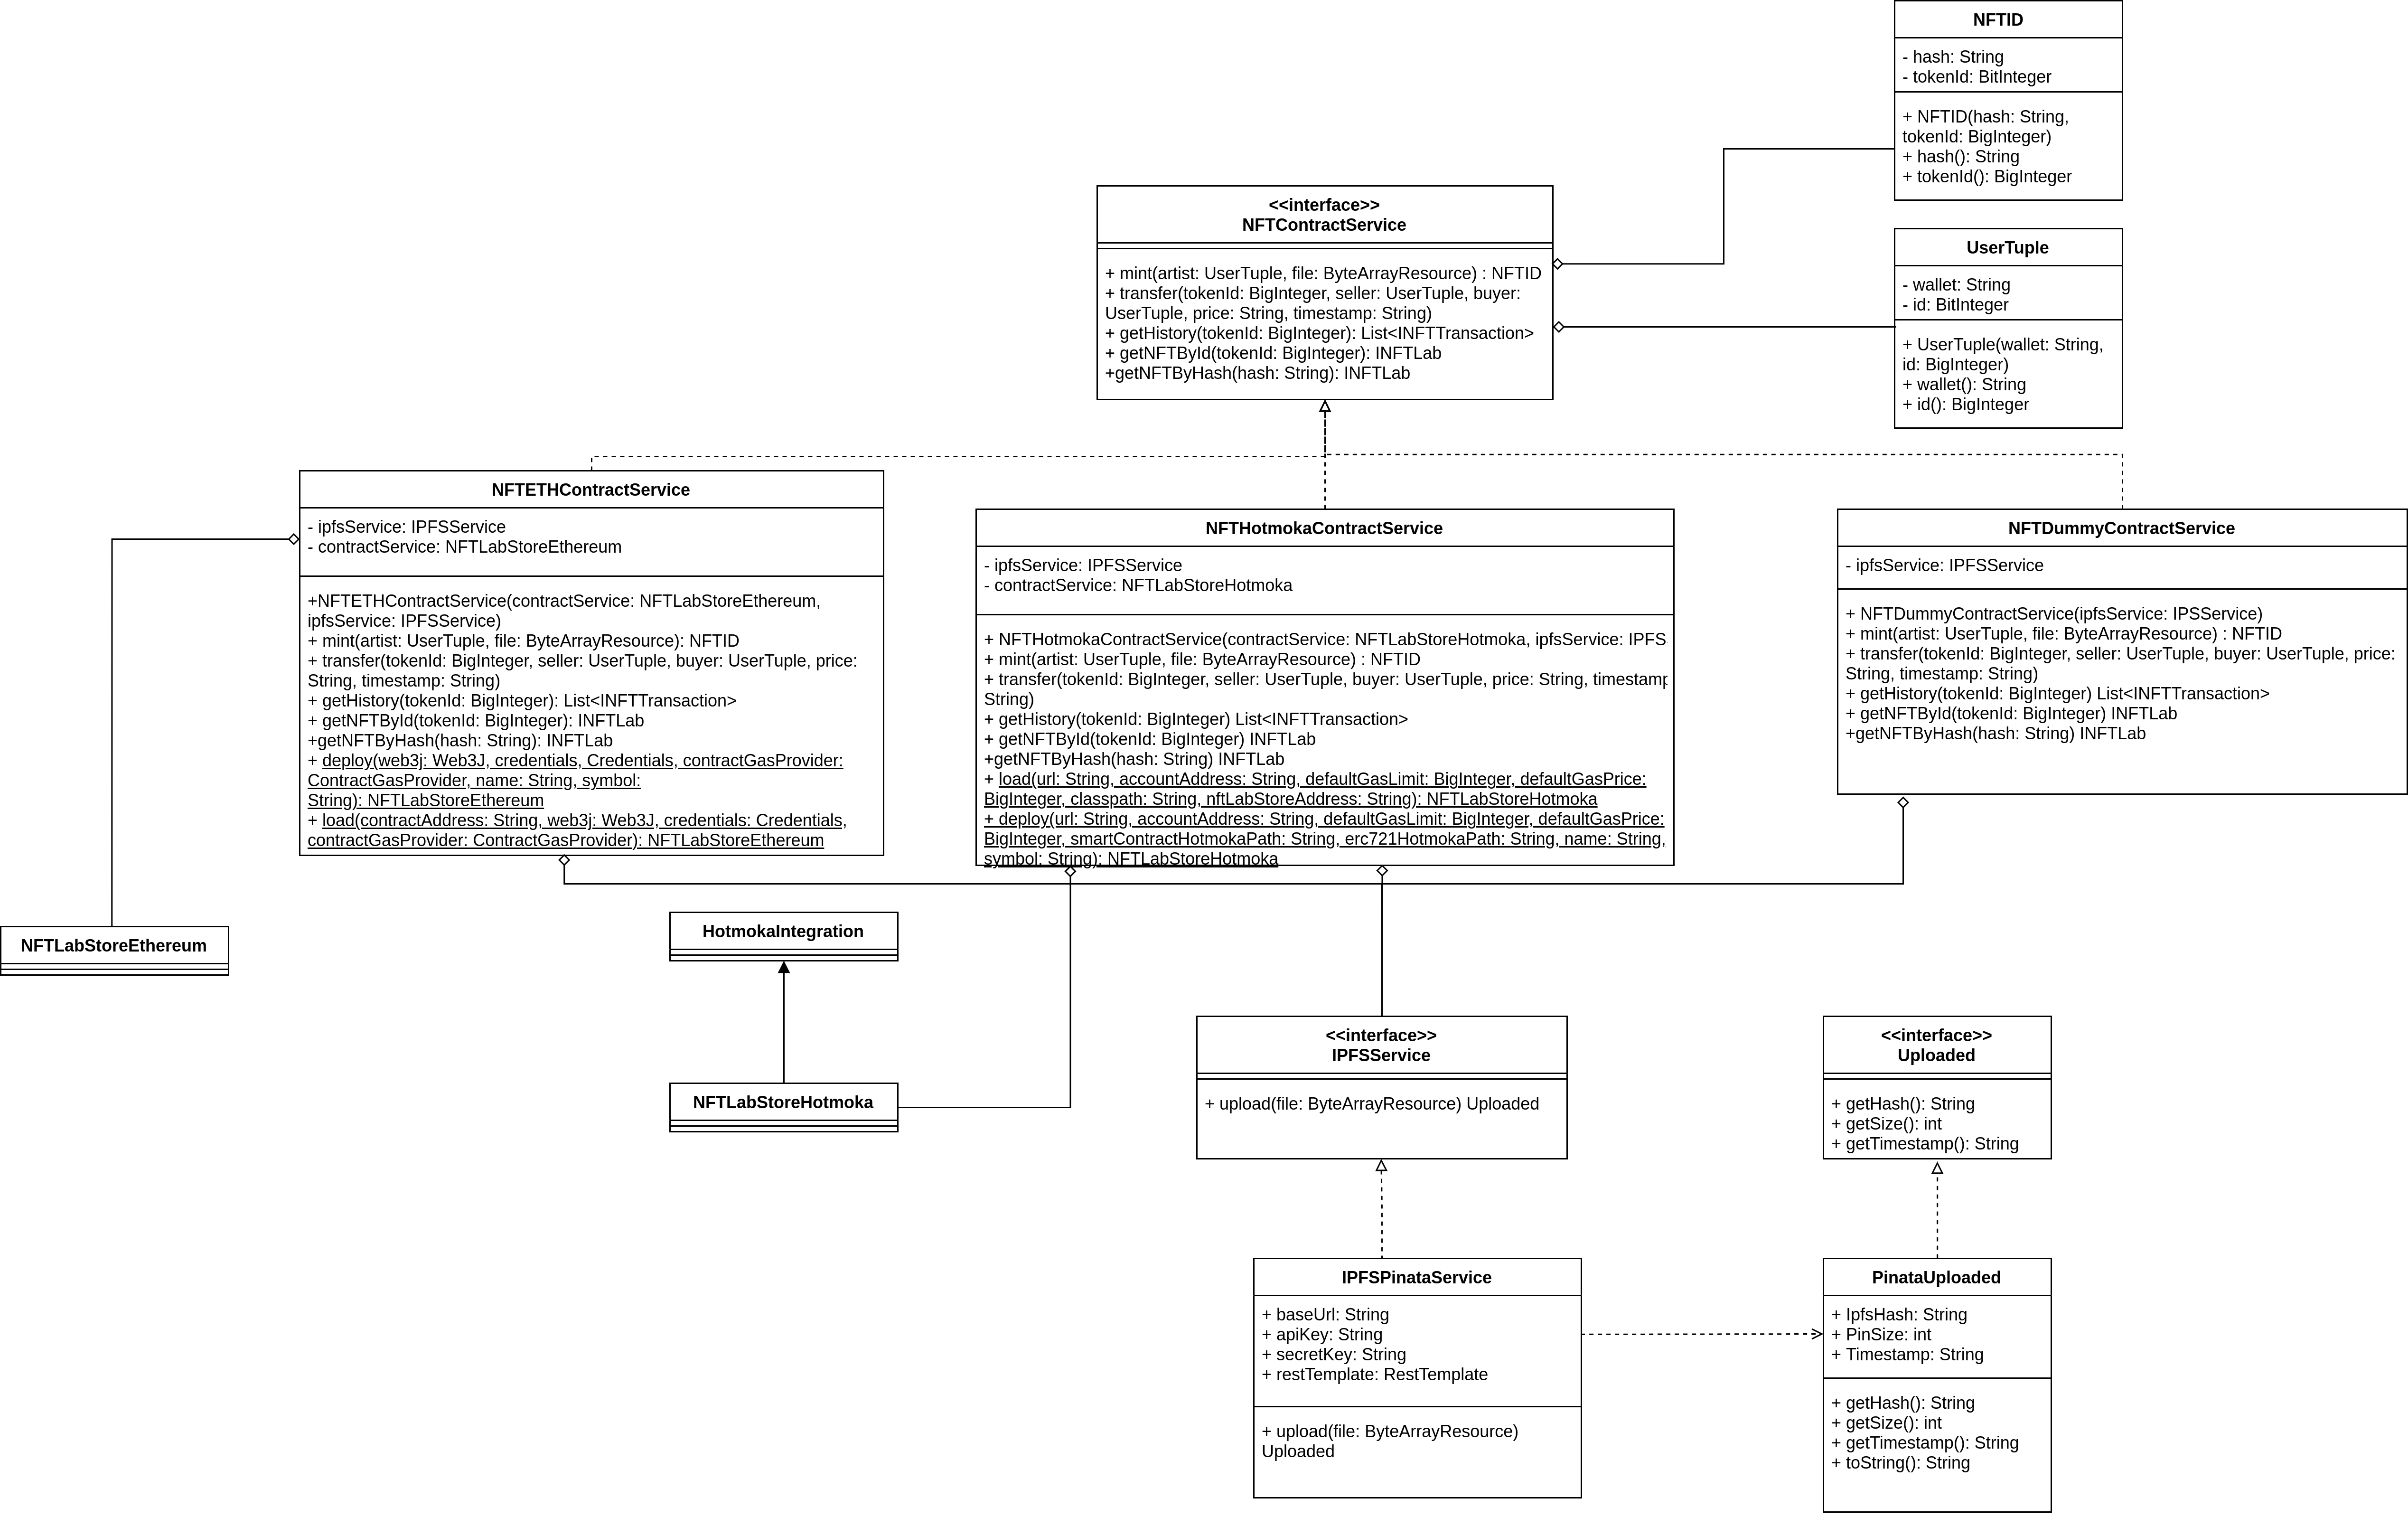
\includegraphics[width=\textwidth]{capitolo3/class-diagram/library-class-diagram.png}
  \caption{Diagramma delle classi della libreria utilizzata per l'integrazione con i contratti}
\end{figure}

\noindent La libreria è stata suddivisa nei seguenti \textit{package}:
\begin{itemize}
  \item \textbf{services}: nel seguente \textit{package} si possono trovare tutti i servizi che permettono al \textit{back-end} di comunicare con la \textit{blockchain} e la rete IPFS, attraverso le classi che ci sono dentro i \textit{package} contracts e services.ipfs;

  \item \textbf{contracts}: nel seguente \textit{package} si possono trovare tutte le classi che hanno il compito di comunicare con le varie \textit{blockchain};

  \item \textbf{services.ipfs}: nel seguente \textit{package} si possono trovare i vari servizi attraverso i quali si può comunicare con la rete IPFS;
  
  \item \textbf{services.smartcontract}: nel seguente \textit{package} si possono trovare tutte le classi che aiutano la gestione dei dati da comunicare con lo \textit{smart contract}.
\end{itemize}

\begin{figure}[h!]
  \centering
  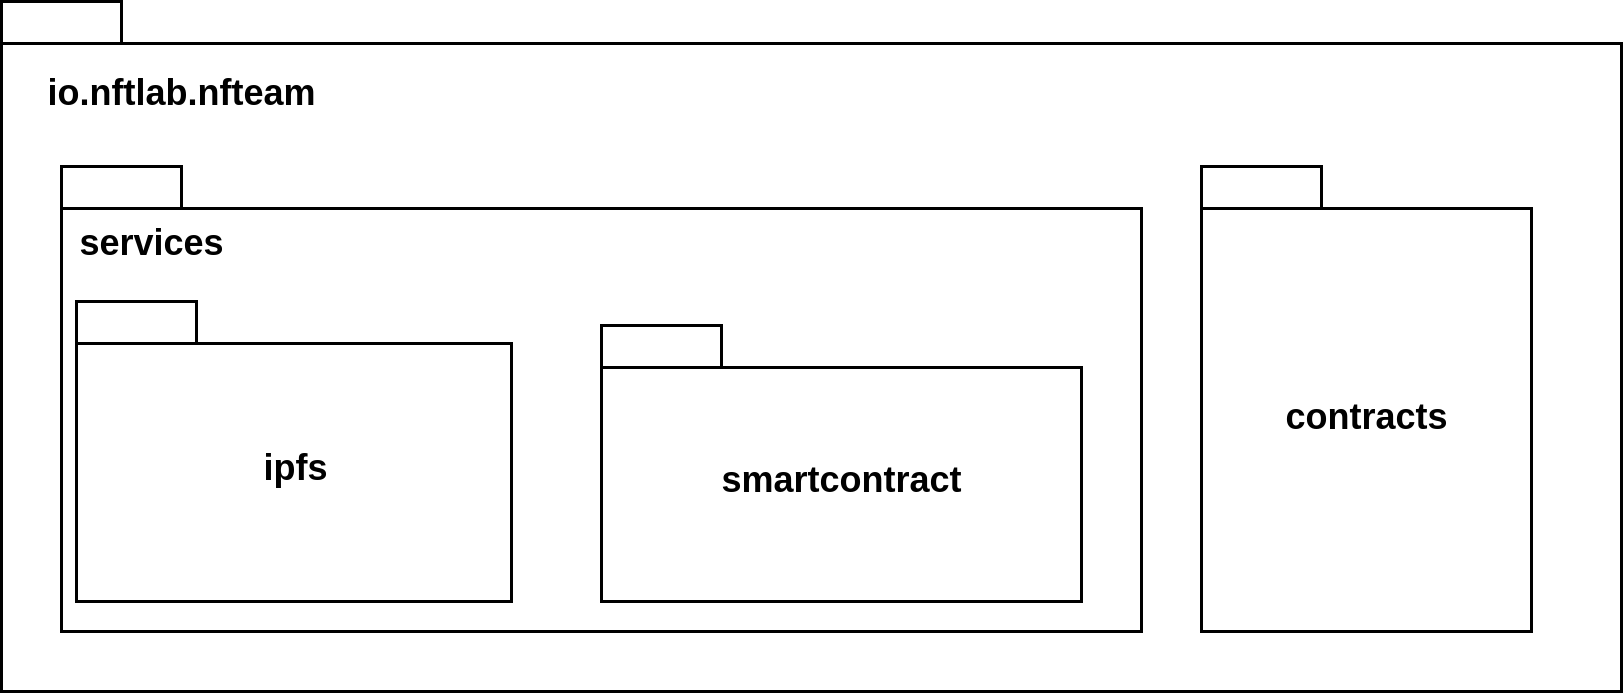
\includegraphics[width=\textwidth]{capitolo3/library/library-packages.png}
  \caption{Diagramma dei \textit{package} della libreria per l'integrazione con i contratti}
\end{figure}

\paragraph{Package services} Per creare una libreria che sia espandibile e che rispetti i principi SOLID, ho fatto uso del \textit{design pattern} chiamato \textit{\textbf{Strategy Pattern}}. Infatti è stata creata un'interfaccia chiamata NFTContractService da cui derivare tutte le specializzazioni per comunicare con qualsiasi \textit{blockchain}, facilmente selezionabili dai \textit{file} di configurazione di Spring nel caso del \textit{back-end} di NFTLab. Sono state create tre specializzazioni:
\begin{itemize}
  \item \textbf{NFTETHContractService}: per comunicare con la rete IPFS e il contratto caricato su \textit{blockchain} Ethereum;
  \item \textbf{NFTHotmokaContractService}: per comunicare con la rete IPFS e il contratto caricato su \textit{blockchain} Hotmoka;
  \item \textbf{NFTDummyContractService}: utilizzata dal \textit{back-end} quando non si vuole comunicare con alcuna \textit{blockchain}, ma solo con la rete IPFS.
\end{itemize}

\paragraph{Package contracts} In questo \textit{package} sono presenti tutte le classi che gestiscono la comunicazione diretta con gli \textit{smart contract}. Per quanto riguarda la classe che gestisce la comunicazione con lo \textit{smart contract} in Ethereum, viene generata automaticamente a partire dal contratto scritto in Solidity attraverso lo strumento Web3J. Al contrario, il contratto per Hotmoka non ha alcuno strumento di questo tipo e per questo ho dovuto provvedere a questa mancanza, attraverso le classi HotmokaIntegration e NFTLabStoreHotmoka. \\

Per l'integrazione con la \textit{blockchain} Hotmoka sono state previste due classi perché HotmokaIntegration ha il compito di gestire tutta la parte di connessione con Hotmoka, mentre in NFTLabStoreHotmoka sono state definite tutte le chiamate che servono per comunicare con il contratto. È stata fatta questa distinzione per separare la logica di connessione alla rete, da quella delle chiamate verso il contratto.

\paragraph{Package services.ipfs} Attraverso il \textit{package} services.ipfs ho definito tutte le classi e interfacce per interagire con la rete IPFS. Sempre grazie all'utilizzo dello \textit{\textbf{Strategy Pattern}} è stata definita l'interfaccia IPFSService, la quale è stata specializzata nella classe \textbf{IPFSPinataService} utilizzata per comunicare con la rete IPFS attraverso il servizio Pinata.

\paragraph{}

A titolo esemplificativo viene riportato il diagramma di sequenza dell'aggiunta di una nuova opera, con annessa creazione di NFT, e quello del trasferimento di proprietà di un NFT.

\begin{figure}[h!]
  \centering
  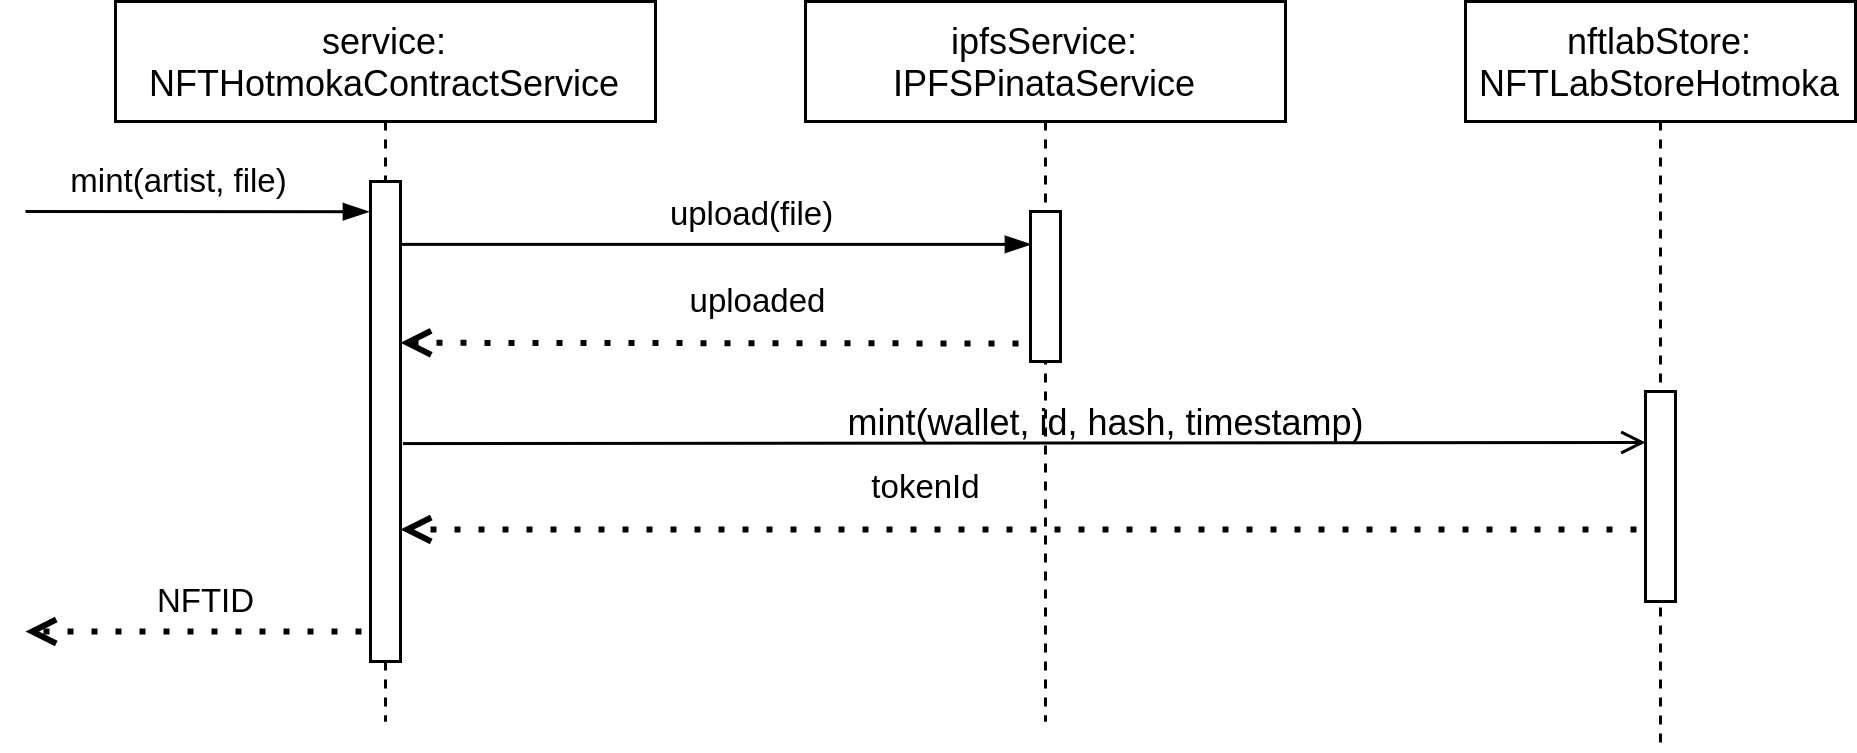
\includegraphics[width=\textwidth]{capitolo3/library/library-activity-creation.png}
  \caption{Diagramma di sequenza del caricamento di un'opera e generazione del NFT}
\end{figure}

\begin{figure}[h!]
  \centering
  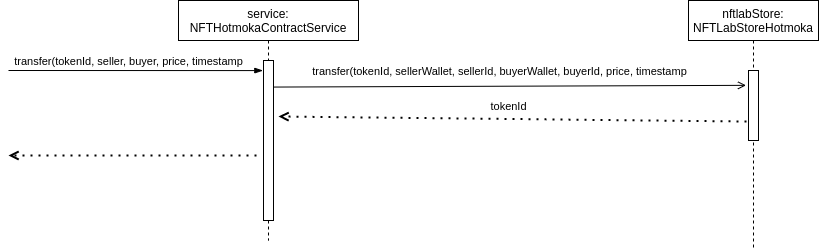
\includegraphics[width=\textwidth]{capitolo3/library/library-activity-transfer.png}
  \caption{Diagramma di sequenza del trasferimento di un NFT}
\end{figure}

\subsection{Codifica}
A partire dalla progettazione architetturale, l'iter di sviluppo si è svolto nel seguente modo:
\begin{enumerate}
  \item implementazione del \textit{package} \textbf{services} e \textbf{services.smartcontract}, dove mi sono concentrato nella scrittura delle classi principali che hanno il compito di comunicare direttamente con il \textit{back-end};
  \item implementazione del \textit{package} \textbf{services.ipfs} e \textbf{services.ipfs.pinataresponses}, dove ho sviluppato il servizio per comunicare con la rete IPFS attraverso Pinata;
  \item implementazione del \textit{package} \textbf{contracts}, dove ho provveduto a generare la classe per comunicare con il contratto caricato su \textit{blockchain} Ethereum e a scrivere il sistema per la comunicazione con la \textit{blockchain} Hotmoka.
\end{enumerate}
% \clearpage
\begin{figure}[h!]
  \centering
  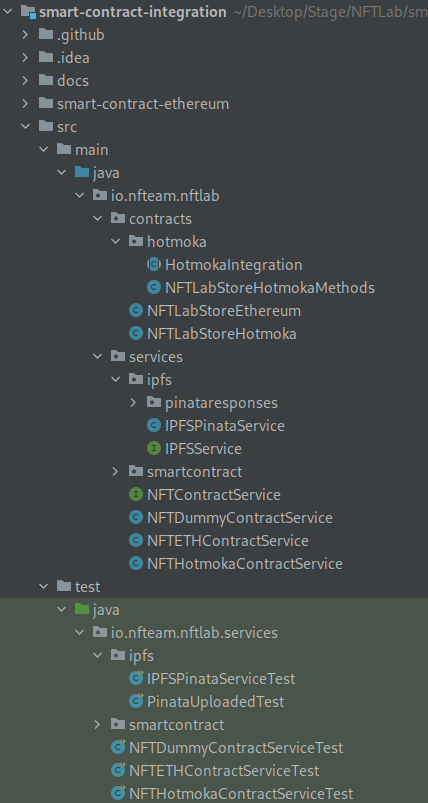
\includegraphics[width=0.35\textwidth]{capitolo3/library/library-structure.png}
  \caption{Struttura del progetto della libreria per l'integrazione con i contratti}
\end{figure}

\subsection{Verifica}
In parallelo con l'attività di codifica, ho verificato lo sviluppo delle libreria sfruttando il \textit{framework} \textbf{JUnit5} e la libreria \textbf{Mockito}. Questi ultimi si integrano perfettamente con lo strumento Maven. \\

Per quanto riguarda i tipi di test eseguiti, sono stati sviluppati quelli di unità, di integrazione e di sistema.

% \clearpage
\begin{figure}[h!]
  \centering
  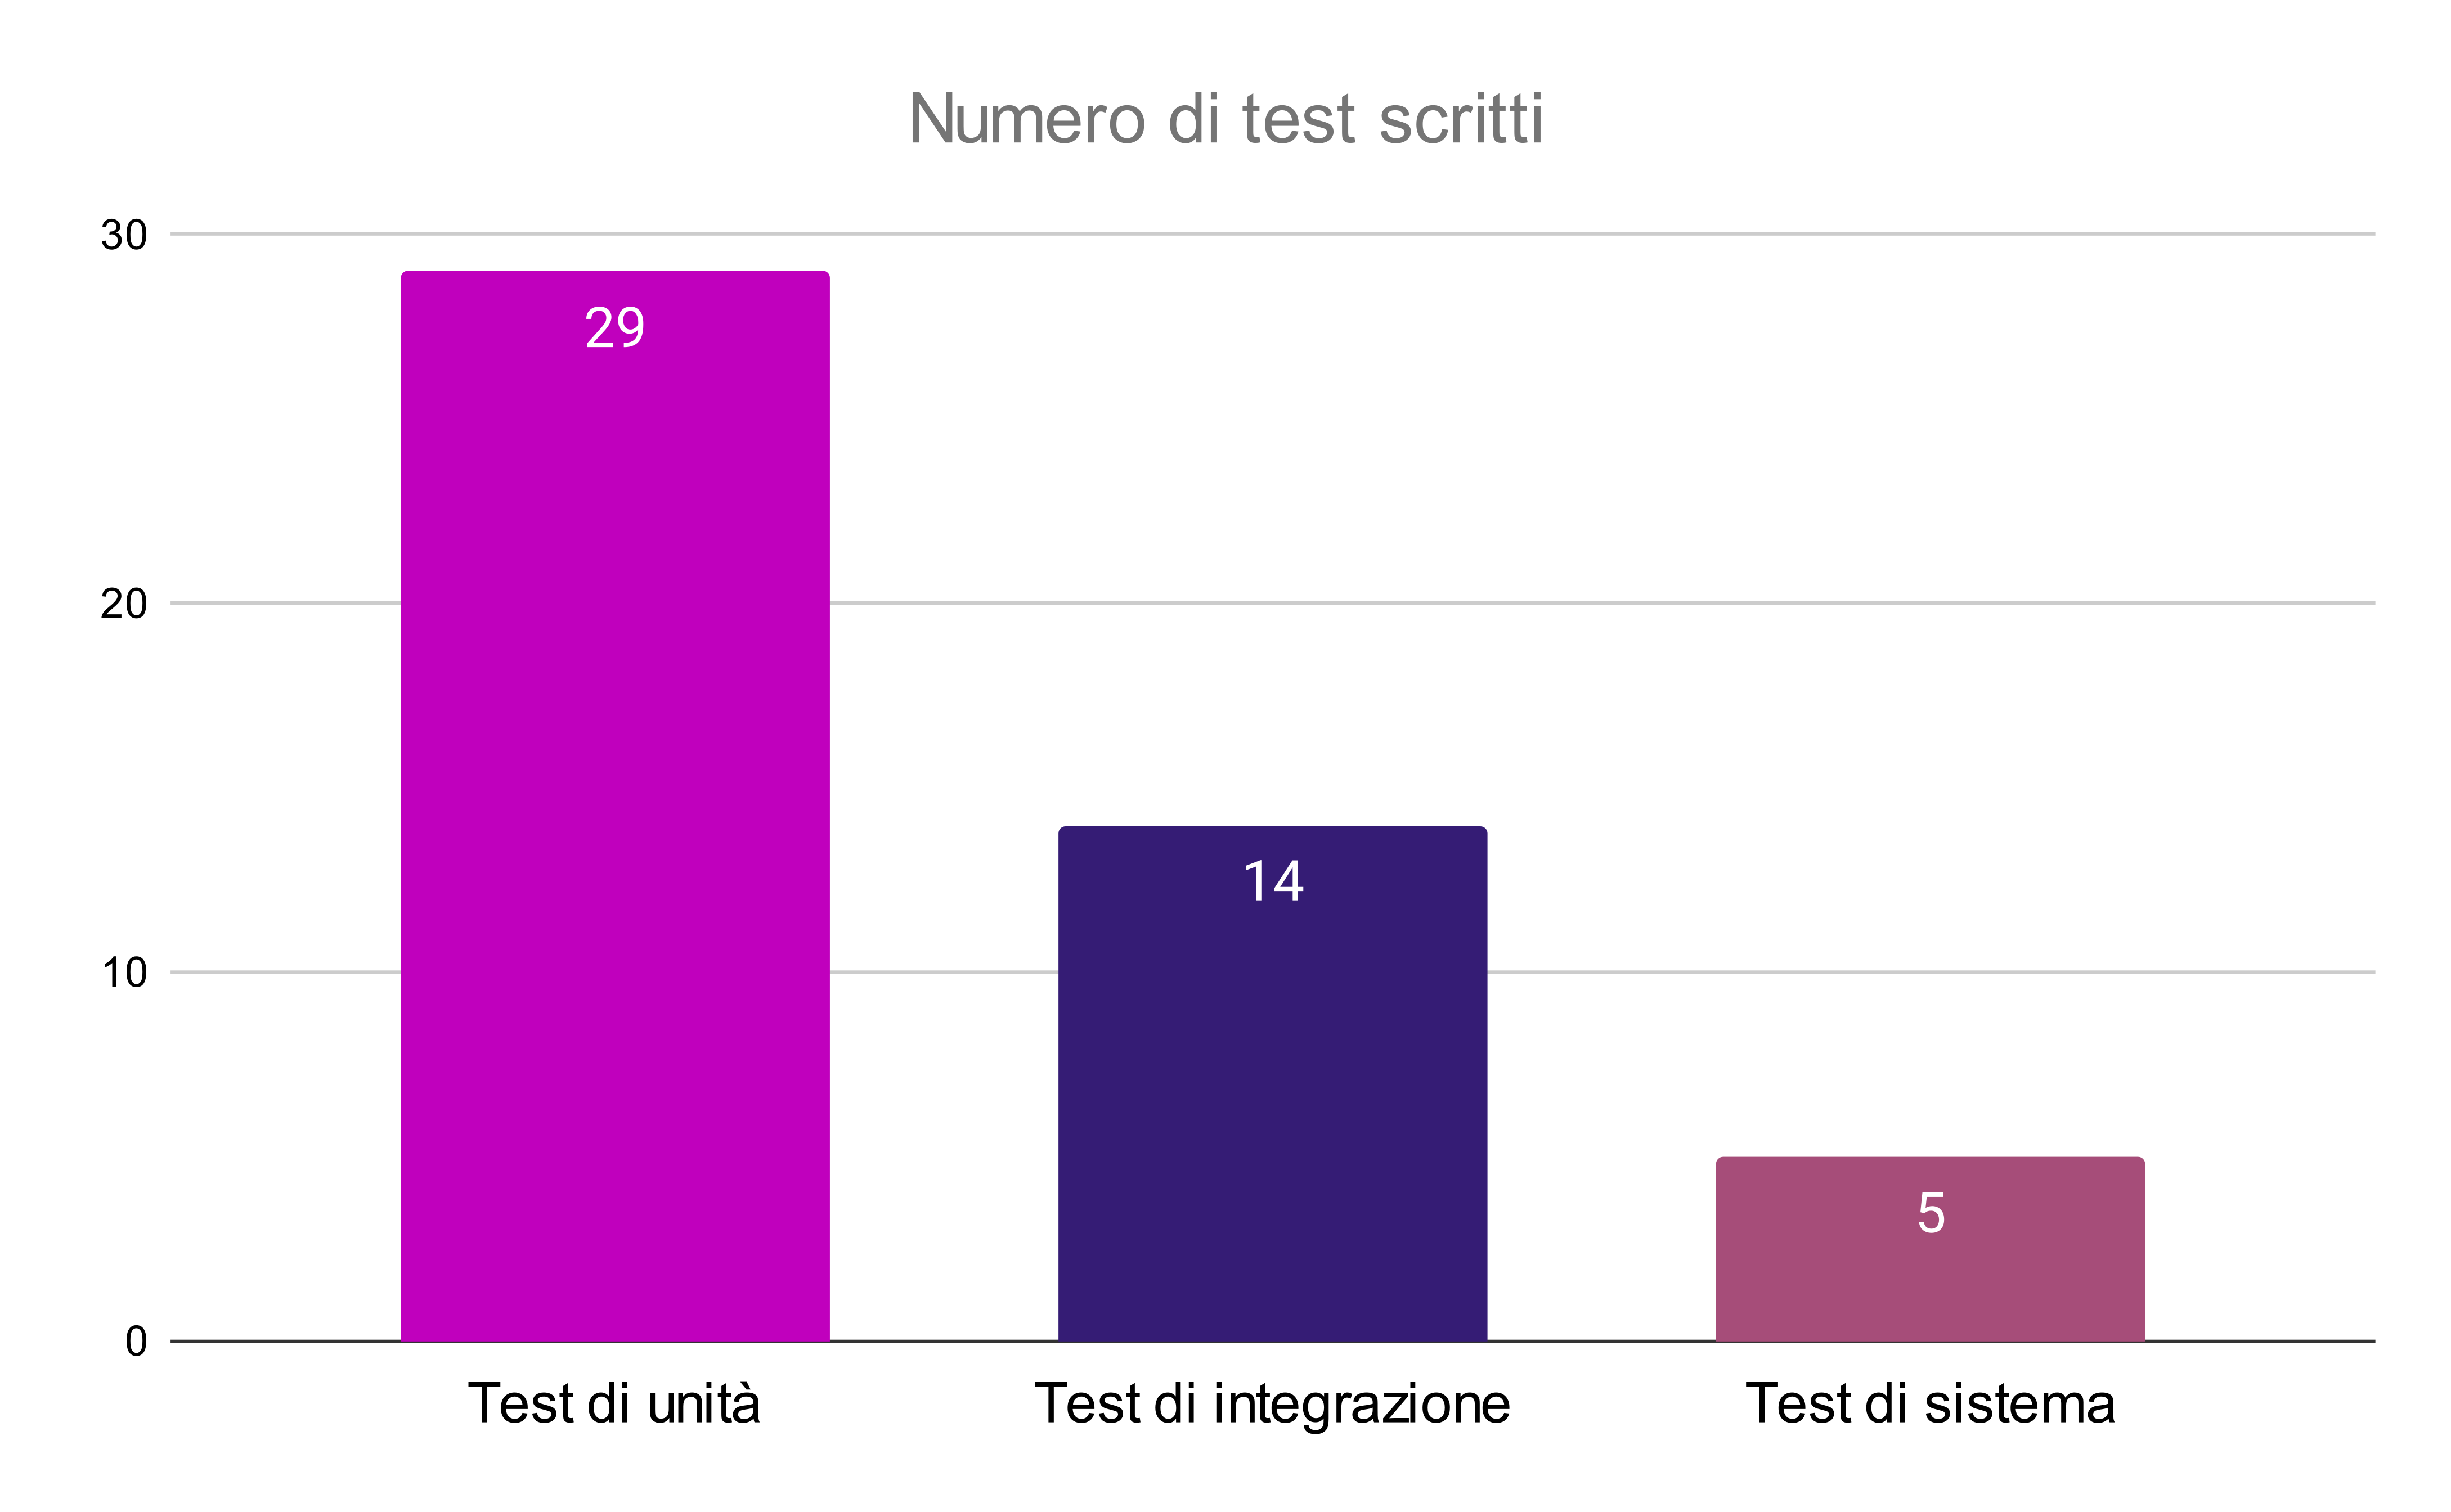
\includegraphics[width=0.8\textwidth]{capitolo3/library-number-test.png}
  \caption{Numero di test scritti nella libreria per l'integrazione con gli \textit{smart contract}}
\end{figure}

In generale, posso affermare che l'attività di verifica si è rilevata molto proficua e mi ha permesso di agevolare lo sviluppo in modo significativo, tanto da produrre un grande quantitativo di \textit{test} e raggiungere un \textit{code coverage} del 90\%.

\begin{figure}[h!]
  \centering
  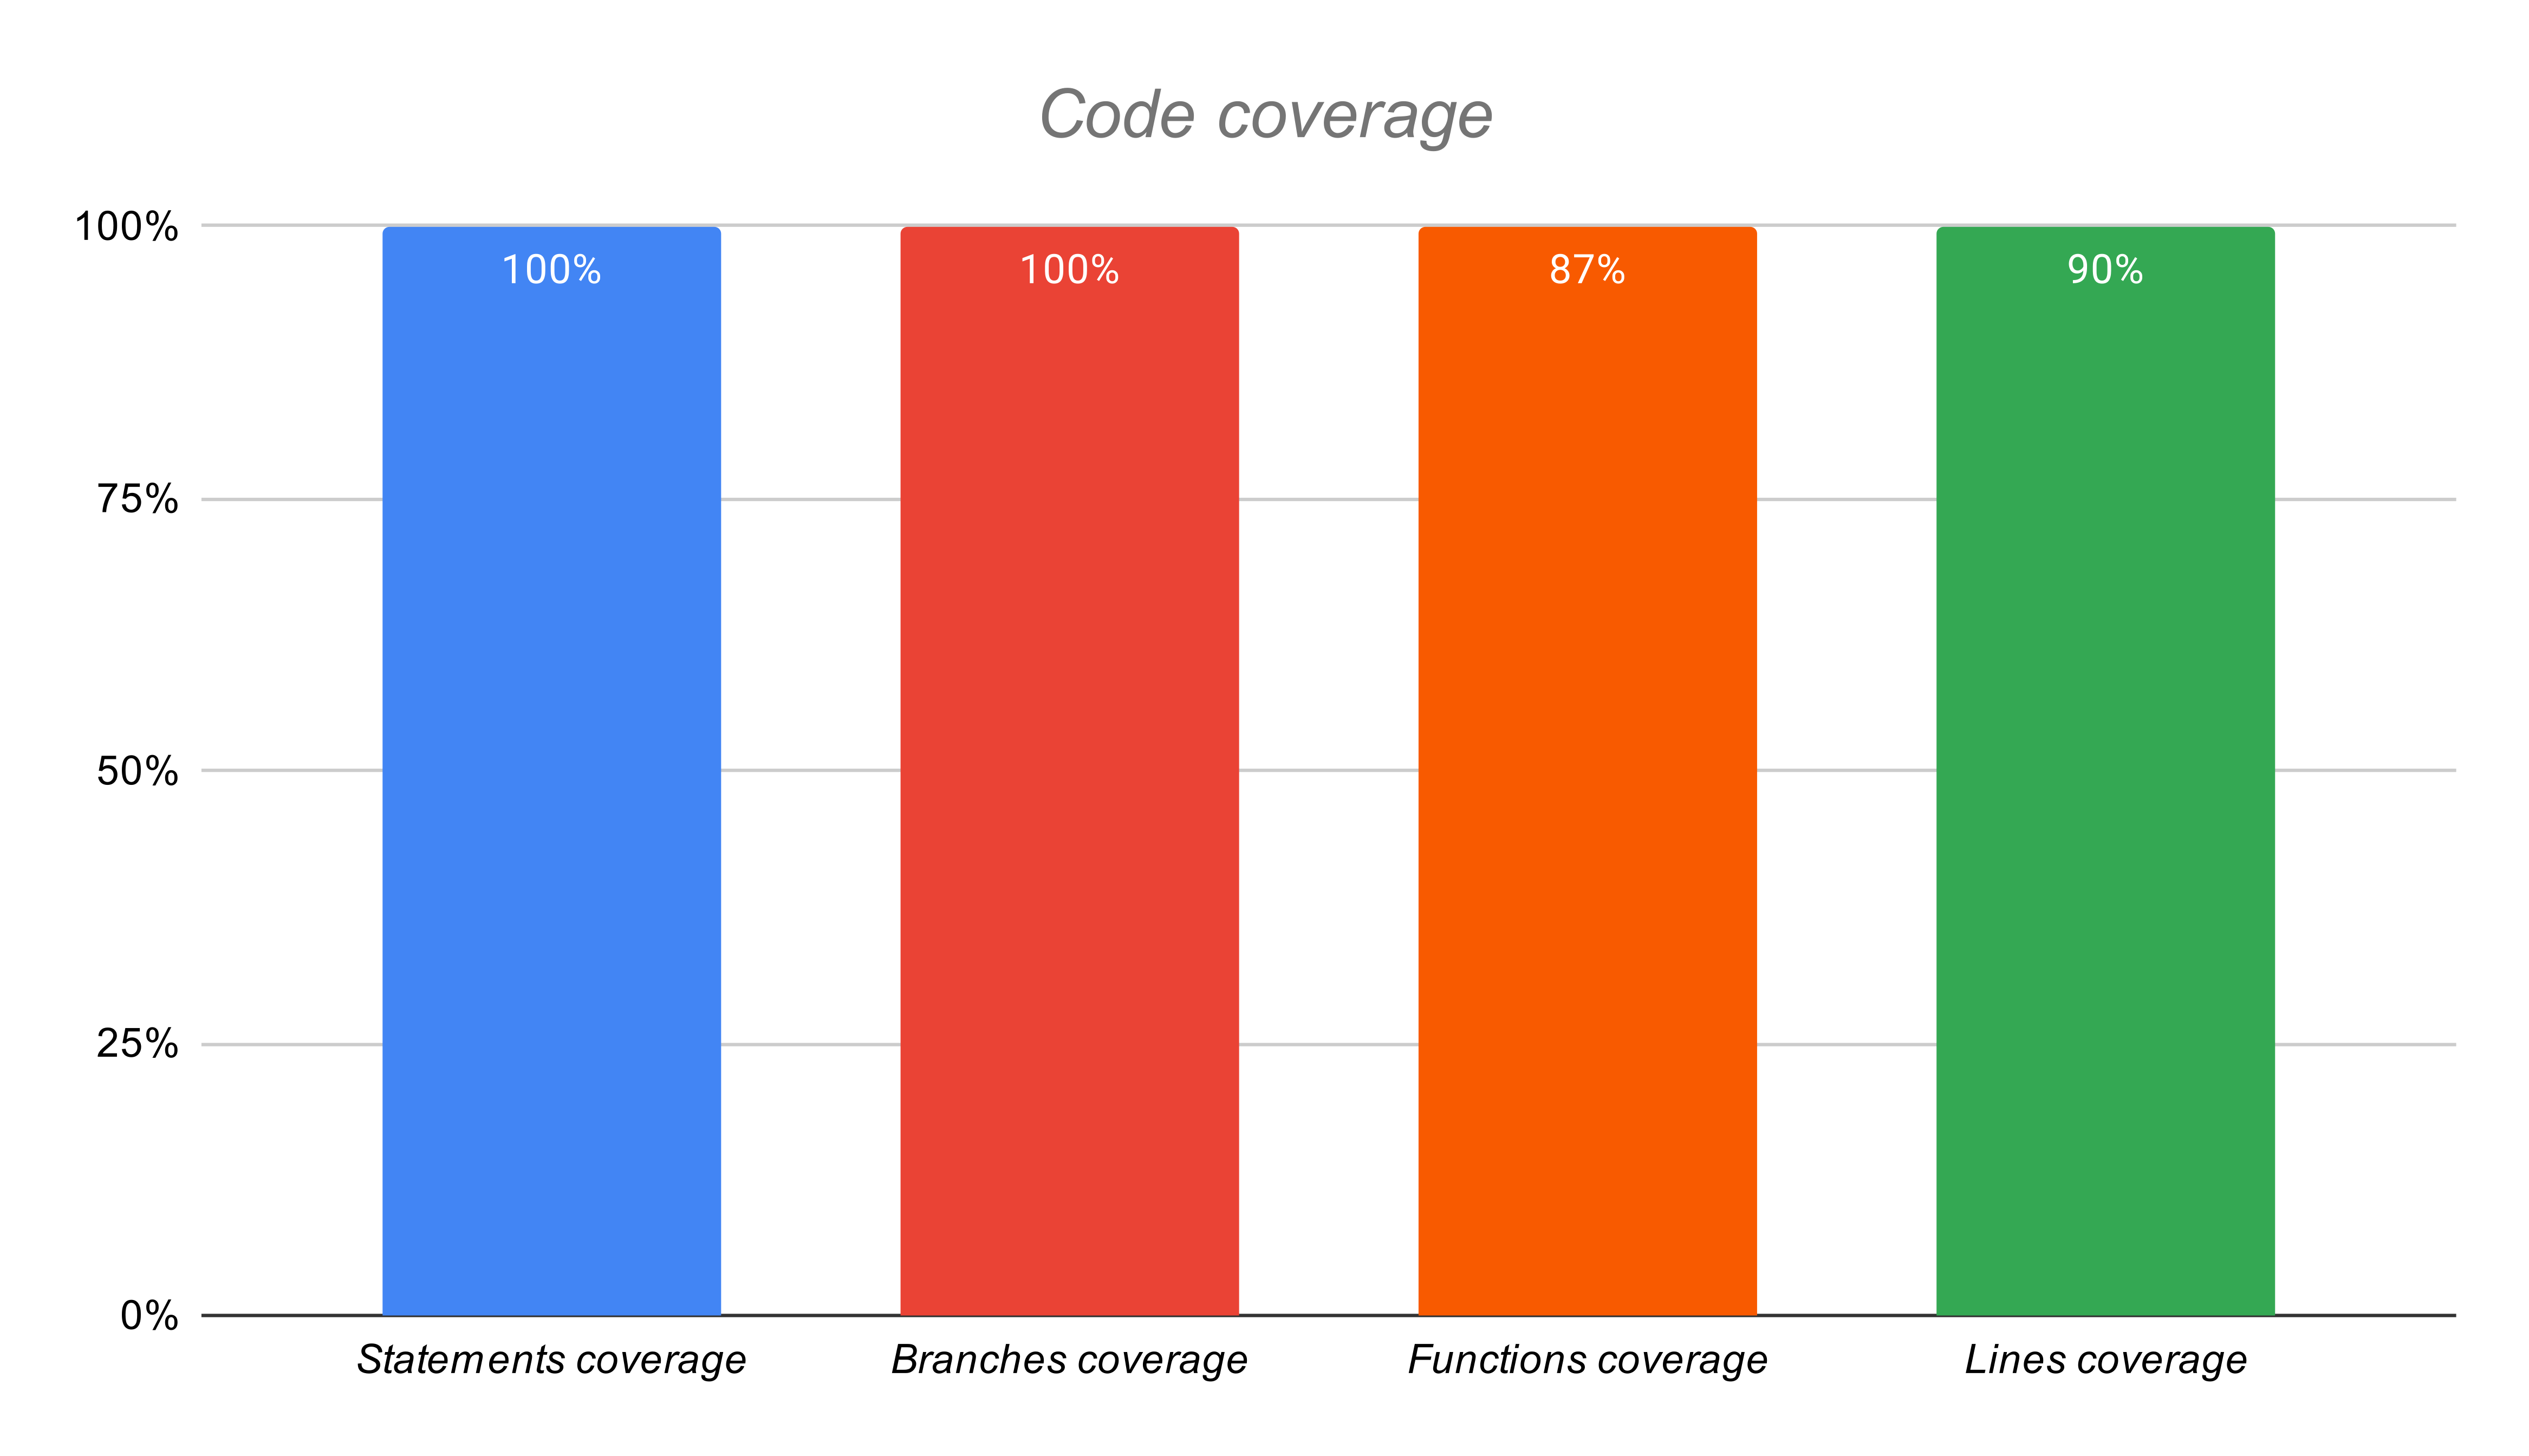
\includegraphics[width=0.8\textwidth]{capitolo3/library-code-coverage.png}
  \caption{\textit{Code coverage} raggiunto nella libreria per l'integrazione con gli \textit{smart contract}}
\end{figure}
